\documentclass[
	9pt, % Set the default font size, options include: 8pt, 9pt, 10pt, 11pt, 12pt, 14pt, 17pt, 20pt
	t, % Uncomment to vertically align all slide content to the top of the slide, rather than the default centered
	%aspectratio=169, % Uncomment to set the aspect ratio to a 16:9 ratio which matches the aspect ratio of 1080p and 4K screens and projectors
]{beamer}

\graphicspath{{Images/}{./}} % Specifies where to look for included images (trailing slash required)

\usepackage{booktabs} % Allows the use of \toprule, \midrule and \bottomrule for better rules in tables
\usepackage{graphicx}
\usepackage{caption}
\usepackage{subcaption}
\usepackage{hyperref}
\usepackage[english,brazil]{babel}
\usepackage{fontawesome5}
\usepackage{listings}
\usepackage{minted}
\usepackage{xcolor}
% \usepackage{graphicx}
% \usepackage{animate}
\RequirePackage[backend=biber,
style=ieee,
citestyle=authoryear,
]{biblatex}

% Define a custom command for an icon link
\newcommand{\iconLink}[2]{\href{#1}{\faLink \hspace{0.2em} {#2}}}
\newcommand{\yellowbox}[1]{\colorbox{yellow!75}{#1}}
\definecolor{darkgreen}{rgb}{0,0.5,0}

% Definindo um estilo para o destaque
%----------------------------------------------------------------------------------------
%	SELECT LAYOUT THEME
%----------------------------------------------------------------------------------------
\usetheme{Madrid}

%----------------------------------------------------------------------------------------
%	SELECT COLOR THEME
%----------------------------------------------------------------------------------------

% Beamer comes with a number of color themes that can be applied to any layout theme to change its colors. Uncomment each of these in turn to see how they change the colors of your selected layout theme.

%\usecolortheme{albatross}
%\usecolortheme{beaver}
%\usecolortheme{beetle}
% \usecolortheme{crane}
%\usecolortheme{dolphin}
%\usecolortheme{dove}
%\usecolortheme{fly}
%\usecolortheme{lily}
%\usecolortheme{monarca}
%\usecolortheme{seagull}
%\usecolortheme{seahorse}
%\usecolortheme{spruce}
%\usecolortheme{whale}
%\usecolortheme{wolverine}

%----------------------------------------------------------------------------------------
%	SELECT FONT THEME & FONTS
%----------------------------------------------------------------------------------------
\usefonttheme{default} % Typeset using the default sans serif font

%------------------------------------------------

\usepackage{palatino} % Use the Palatino font for serif text
\usepackage[default]{lato} % Use the Lato font for sans serif text

%----------------------------------------------------------------------------------------
%	SELECT INNER THEME
%----------------------------------------------------------------------------------------
\useinnertheme{rectangles}

%----------------------------------------------------------------------------------------
%	SELECT OUTER THEME
%----------------------------------------------------------------------------------------

% Outer themes change the overall layout of slides, such as: header and footer lines, sidebars and slide titles. Uncomment each theme in turn to see what changes it makes to your presentation.

%\useoutertheme{default}
%\useoutertheme{infolines}
%\useoutertheme{miniframes}
%\useoutertheme{smoothbars}
%\useoutertheme{sidebar}
%\useoutertheme{split}
%\useoutertheme{shadow}
%\useoutertheme{tree}
%\useoutertheme{smoothtree}

%\setbeamertemplate{footline} % Uncomment this line to remove the footer line in all slides
%\setbeamertemplate{footline}[page number] % Uncomment this line to replace the footer line in all slides with a simple slide count

%\setbeamertemplate{navigation symbols}{} % Uncomment this line to remove the navigation symbols from the bottom of all slides

% \bibliography{references} % Specifies the bibliography file to include publications
% \bibliographystyle{apalike} % Specifies the bibliography style
\addbibresource{references.bib}

%----------------------------------------------------------------------------------------
%	PRESENTATION INFORMATION
%----------------------------------------------------------------------------------------

\title[DesWebII]{Desenvolvimento Web II} % The short title in the optional parameter appears at the bottom of every slide, the full title in the main parameter is only on the title page
\subtitle{Aula 06 - Integração e Entrega Contínua - CI/CD} % Presentation subtitle, remove this command if a subtitle isn't required
\author[Fabricio Bizotto]{Prof. Fabricio Bizotto} % Presenter name(s), the optional parameter can contain a shortened version to appear on the bottom of every slide, while the main parameter will appear on the title slide
\institute[IFC]{Instituto Federal Catarinense \\ \smallskip \textit{fabricio.bizotto@ifc.edu.br}} % Your institution, the optional parameter can be used for the institution shorthand and will appear on the bottom of every slide after author names, while the required parameter is used on the title slide and can include your email address or additional information on separate lines
\date[\today]{Ciência da Computação \\ \today} % Presentation date or conference/meeting name, the optional parameter can contain a shortened version to appear on the bottom of every slide, while the required parameter value is output to the title slide

%----------------------------------------------------------------------------------------
\begin{document}

%----------------------------------------------------------------------------------------
%	TITLE SLIDE
%----------------------------------------------------------------------------------------

\begin{frame}
	\titlepage % Output the title slide, automatically created using the text entered in the PRESENTATION INFORMATION block above
\end{frame}

%----------------------------------------------------------------------------------------
%	TABLE OF CONTENTS SLIDE
%----------------------------------------------------------------------------------------

\begin{frame}
	\frametitle{Roteiro} % Slide title, remove this command for no title
	
	\tableofcontents % Output the table of contents (all sections on one slide)
	%\tableofcontents[pausesections] % Output the table of contents (break sections up across separate slides)
\end{frame}

%----------------------------------------------------------------------------------------
%	PRESENTATION BODY SLIDES
%----------------------------------------------------------------------------------------

\section{Manifesto Ágil}

%------------------------------------------------

\begin{frame}
	\frametitle{Manifesto Ágil}
	\begin{itemize}
		\item O Manifesto Ágil foi escrito em 2001 por 17 desenvolvedores de software que se reuniram para discutir métodos leves de desenvolvimento de software.
		\item O Manifesto Ágil é baseado em 4 valores e 12 princípios.
		\item Os 4 valores do Manifesto Ágil são:
		\begin{enumerate}
			\item Indivíduos e interações mais que processos e ferramentas;
			\item Software em funcionamento mais que documentação abrangente;
			\item Colaboração com o cliente mais que negociação de contratos;
			\item Responder a mudanças mais que seguir um plano.
		\end{enumerate}
	\end{itemize}
\end{frame}

\section{Integração Contínua} % Sections are added in order to organize your presentation into discrete blocks, all sections and subsections are automatically output to the table of contents as an overview of the talk but NOT output in the presentation as separate slides

%------------------------------------------------

\begin{frame}
	\frametitle{Integração Contínua - \textit{Continuous Integration (CI)}}
	\begin{itemize}
		\item CI é uma \yellowbox{prática} de desenvolvimento de software em que os desenvolvedores integram \yellowbox{pequenos pedaços} de código em um repositório compartilhado \yellowbox{frequentemente}, de preferência várias vezes ao dia.
		\item Cada integração é verificada por uma \yellowbox{\textbf{build} automatizada} (incluindo testes) para detectar erros de integração o mais rápido possível.
		\item Esse tipo de abordagem leva a uma redução significativa nos problemas de integração e permite que uma equipe desenvolva software coeso mais rapidamente.
		\item O CI pode ser falhar por: \textbf{builds} quebradas, testes quebrados, cobertura de testes insuficiente, etc.
	\end{itemize}

	\begin{block}{Pipeline - Fluxo de Trabalho}
		\begin{enumerate}
			\item \textbf{Controle de Versão}: Desenvolvedor faz \textbf{commit} no repositório compartilhado;
			\item \textbf{Gatilho Automático}: Servidor de CI monitora o repositório e faz o \textbf{pull} do código;
			\item \textbf{Compilação e Testes Automatizados}: Servidor de CI executa a \textbf{build} e os testes;
			\item \textbf{Relatório}: Servidor de CI notifica o desenvolvedor sobre o resultado. 
		\end{enumerate}
	\end{block}

\end{frame}

%------------------------------------------------

\begin{frame}
	\frametitle{Integração Contínua}
	\begin{figure}
		\centering
		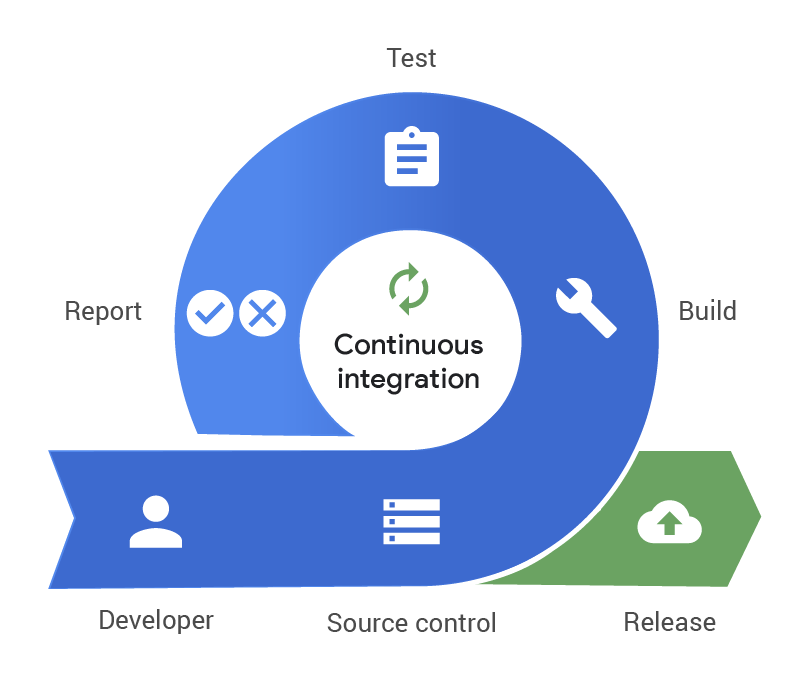
\includegraphics[width=0.7\linewidth]{cont_integ.png}
		\caption{Integração Contínua}
		\label{fig:ci}
	\end{figure}

\end{frame}

%------------------------------------------------

\section{Entrega Contínua}

%------------------------------------------------

\begin{frame}
	\frametitle{Entrega Contínua - \textit{Continuous Delivery (CD)}}
	\begin{itemize}
		\item CD é uma abordagem de engenharia de software na qual as equipes produzem software em ciclos curtos, garantindo que o software possa ser implantado de forma confiável a qualquer momento.
		\item CD visa garantir que um aplicativo esteja sempre no estado pronto para produção após passar com sucesso em testes automatizados e verificações de qualidade.
		\item O CD visa tornar o processo de implantação automatizado, de modo que qualquer alteração no software possa ser implantada de forma rápida e segura.
		\item O CD pode falhar por: \textbf{builds} quebradas, testes quebrados, cobertura de testes insuficiente, etc.
	\end{itemize}

\end{frame}


\begin{frame}
	\frametitle{Pipeline de Integração e Entrega Contínua}
	\begin{figure}
		\centering
		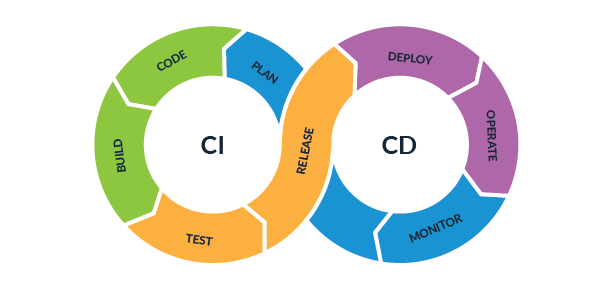
\includegraphics[width=0.9\linewidth]{ci_cd_pipeline.png}
		\caption{Pipeline de Integração e Entrega Contínua}
		\label{fig:ci_cd}
	\end{figure}
\end{frame}

\begin{frame}
	\frametitle{Pipeline de Integração e Entrega Contínua}
	
	\begin{itemize}
		\item O pipeline introduz monitoramento e automação para melhoria no processo de desenvolvimento de software, principalmente nas fases de integração e teste.
		\item Embora seja possível executar o pipeline manualmente, o objetivo é que ele seja executado automaticamente sempre que houver uma alteração no código.
	\end{itemize}
	\begin{block}{Pipeline - Fluxo de Trabalho}
		As etapas típicas de um pipeline de CI/CD são:
		\bigskip

		\begin{enumerate}
			\item \textbf{Teste}: Testes unitários, testes de integração, testes de aceitação, etc;
			\item \textbf{Build}: Compilação, empacotamento, etc;
			\item \textbf{Release}: Implantação em ambientes de homologação e produção;
			\item \textbf{Monitoramento}: Monitoramento de desempenho, disponibilidade, etc.
			\item \textbf{Feedback}: Notificação de falhas, relatórios de desempenho, etc. 
		\end{enumerate}
	\end{block}
		
\end{frame}

\section{Ferramentas}

\begin{frame}
	\frametitle{Ferramentas}
	\begin{itemize}
		\item \textbf{Ferramentas básicas}: Git, GitHub, Docker, Docker Hub;
		\item \textbf{CI/CD}: GitLab, Jenkins, Circle CI, GitHub Actions, GoCD, Semaphore, Travis CI;
		\item \textbf{Cloud}: AWS, Azure, Google Cloud, Heroku, Digital Ocean, Surge, GitHub Pages, Netlify, Vercel, etc.
		\item \textbf{Monitoramento}: New Relic, Datadog, AppDynamics, etc.
		\item \textbf{Testes}: Selenium, Cypress, Jest, JUnit, Vitest, etc.
		\item \textbf{Cobertura de Testes}: Istanbul, Jacoco, SonarQube, etc.
		\item \textbf{Análise de Código}: SonarQube, Codacy, Code Climate, etc.
	\end{itemize}

\end{frame}

\section{Exemplo}

\begin{frame}
	\begin{center}
		
		\bigskip\bigskip\bigskip\bigskip % Vertical whitespace
		{\Large Integração Contínua}
		
		\bigskip\bigskip % Vertical whitespace
		{\Huge Exemplo prático}
		
		\bigskip \bigskip
		{\small Vamos ver um exemplo prático de CI/CD usando o GitHub Actions}\\
		{\small \iconLink{https://github.com/fabricioifc/ci-cd-example}{https://github.com/fabricioifc/ci-cd-example}}
	\end{center}

\end{frame}

\section{QUIZ}

\begin{frame}
	\frametitle{QUIZ}
	\framesubtitle{Questão 1/5}

	{\Large O que é Integração Contínua (CI)?}

	\begin{exampleblock}{Resposta}
		\begin{enumerate}[a]
			\item Um processo que integra diferentes sistemas em uma única aplicação.
			\item Um método para integrar continuamente novos recursos em uma aplicação.
			\item Uma prática que visa integrar e testar automaticamente as alterações no código fonte.
		\end{enumerate}
	\end{exampleblock}

\end{frame}

\begin{frame}
	\frametitle{QUIZ}
	\framesubtitle{Questão 1/5}

	{\Large O que é Integração Contínua (CI)?}

	\begin{exampleblock}{Resposta}
		\begin{enumerate}[a]
			\item Um processo que integra diferentes sistemas em uma única aplicação.
			\item Um método para integrar continuamente novos recursos em uma aplicação.
			\item \textcolor{darkgreen}{Uma prática que visa integrar e testar automaticamente as alterações no código fonte.}
		\end{enumerate}
	\end{exampleblock}

\end{frame}

\begin{frame}
	\frametitle{QUIZ}
	\framesubtitle{Questão 2/5}

	{\Large Qual é o principal objetivo da Integração Contínua?}

	\begin{exampleblock}{Resposta}
		\begin{enumerate}[a]
			\item Garantir que as alterações no código sejam integradas e testadas frequentemente.
			\item Reduzir o número de desenvolvedores na equipe.
			\item Aumentar o tempo entre as versões da aplicação.
		\end{enumerate}
	\end{exampleblock}

\end{frame}

\begin{frame}
	\frametitle{QUIZ}
	\framesubtitle{Questão 2/5}

	{\Large Qual é o principal objetivo da Integração Contínua?}

	\begin{exampleblock}{Resposta}
		\begin{enumerate}[a]
			\item \textcolor{darkgreen}{Garantir que as alterações no código sejam integradas e testadas frequentemente.}
			\item Reduzir o número de desenvolvedores na equipe.
			\item Aumentar o tempo entre as versões da aplicação.
		\end{enumerate}
	\end{exampleblock}

\end{frame}

\begin{frame}
	\frametitle{QUIZ}
	\framesubtitle{Questão 3/5}

	{\Large Qual é a diferença entre Integração Contínua e Entrega Contínua? }

	\begin{exampleblock}{Resposta}
		\begin{enumerate}[a]
			\item Não há diferença, os termos são usados de forma intercambiável.
			\item Entrega Contínua é apenas uma fase avançada da Integração Contínua.
			\item Integração Contínua se refere à integração frequente de código, enquanto Entrega Contínua envolve a entrega automatizada de software funcional.
		\end{enumerate}
	\end{exampleblock}

\end{frame}

\begin{frame}
	\frametitle{QUIZ}
	\framesubtitle{Questão 3/5}

	{\Large Qual é a diferença entre Integração Contínua e Entrega Contínua? }

	\begin{exampleblock}{Resposta}
		\begin{enumerate}[a]
			\item Não há diferença, os termos são usados de forma intercambiável.
			\item Entrega Contínua é apenas uma fase avançada da Integração Contínua.
			\item \textcolor{darkgreen}{Integração Contínua se refere à integração frequente de código, enquanto Entrega Contínua envolve a entrega automatizada de software funcional.}
		\end{enumerate}
	\end{exampleblock}

\end{frame}

\begin{frame}
	\frametitle{QUIZ}
	\framesubtitle{Questão 4/5}

	{\Large Qual é a importância dos testes automatizados na Integração Contínua? }

	\begin{exampleblock}{Resposta}
		\begin{enumerate}[a]
			\item Não são necessários, pois a Integração Contínua já cobre todos os aspectos.
			\item Garantir que as alterações no código não quebrem funcionalidades existentes.
			\item Apenas agilizar o processo de integração, sem impacto na qualidade do software.
		\end{enumerate}
	\end{exampleblock}

\end{frame}

\begin{frame}
	\frametitle{QUIZ}
	\framesubtitle{Questão 4/5}

	{\Large Qual é a importância dos testes automatizados na Integração Contínua? }

	\begin{exampleblock}{Resposta}
		\begin{enumerate}[a]
			\item Não são necessários, pois a Integração Contínua já cobre todos os aspectos.
			\item \textcolor{darkgreen}{Garantir que as alterações no código não quebrem funcionalidades existentes.}
			\item Apenas agilizar o processo de integração, sem impacto na qualidade do software.
		\end{enumerate}
	\end{exampleblock}

\end{frame}

\begin{frame}
	\frametitle{QUIZ}
	\framesubtitle{Questão 5/5}

	{\Large Quais benefícios podem ser obtidos ao implementar a Integração Contínua? }

	\begin{exampleblock}{Resposta}
		\begin{enumerate}[a]
			\item Maior número de bugs.
			\item Maior confusão entre os membros da equipe.
			\item Detectar e corrigir problemas de integração mais cedo, facilitando o desenvolvimento contínuo e a entrega de software de alta qualidade.
		\end{enumerate}
	\end{exampleblock}

\end{frame}

\begin{frame}
	\frametitle{QUIZ}
	\framesubtitle{Questão 5/5}

	{\Large Quais benefícios podem ser obtidos ao implementar a Integração Contínua? }

	\begin{exampleblock}{Resposta}
		\begin{enumerate}[a]
			\item Maior número de bugs.
			\item Maior confusão entre os membros da equipe.
			\item \textcolor{darkgreen}{Detectar e corrigir problemas de integração mais cedo, facilitando o desenvolvimento contínuo e a entrega de software de alta qualidade.}
		\end{enumerate}
	\end{exampleblock}

\end{frame}

%------------------------------------------------

\section{Experimentos}

\begin{frame}
	\frametitle{Experimentos}
	\begin{itemize}
		\item \textbf{Experimento 1}\\ Siga \href{https://github.com/fabricioifc/ci-cd-example/blob/main/README.md}{\textcolor{blue}{esse passo a passo}} para criar um repositório no GitHub e configurar o GitHub Actions para executar os testes e o deploy de forma automática no GitHub Pages.
		\item \textbf{Experimento 2}\\ Faça alterações no código e observe o resultado no GitHub Actions.
		\item \textbf{Experimento 3}\\ Faça alterações que quebrem os testes e observe o resultado no GitHub Actions.
	\end{itemize}

	\begin{block}{Desafio}
		\begin{itemize}
			\item Crie um novo projeto que faça uso de CI/CD e publique no GitHub.
			\item Use o GitHub Actions ou outra ferramenta de CI/CD.
			\item Use o GitHub Pages ou outra ferramenta de hospedagem.
			\item Crie um ambiente de homologação e um de produção. 
			\item Faça uso de testes automatizados.
		\end{itemize}

	\end{block}

\end{frame}


\end{document} 
